%\documentclass[letterpaper]{scrartcl}
%\documentclass[letterpaper,10pt]{scrartcl}
\documentclass[letterpaper,oneside,10pt]{scrbook}
\usepackage[body={5.8in,8.5in},
  top=1.2in, left=1.4in]{geometry}
%\usepackage[body={4.8in,7.5in},
%  top=1.2in, left=1.8in]{geometry}
\usepackage{xcolor}
\usepackage{mathptmx}
\usepackage{helvet}
%\usepackage{mathpazo}
%\usepackage{fourier}
%\usepackage{lmodern}
% listings --
\usepackage{listings}
\newcommand{\passthrough}[1]{#1}
\definecolor{listing-text-background}{HTML}{F7F7F7}
\definecolor{listing-text-rule}{HTML}{B3B2B3}
\definecolor{listing-renumf90-background}{HTML}{EFEFFE}
\definecolor{listing-blupf90-background}{HTML}{E7FFE7}
\definecolor{listing-blupf90-rule}{HTML}{B3B2B3}
\definecolor{listing-blupf90-keyword}{HTML}{435489}
\definecolor{listing-blupf90-comment}{HTML}{8E8E8E}
\lstdefinelanguage{blupf90}{
  style={parameterfile},
  morekeywords={
    OPTION
  },
  sensitive=false,
  morecomment=[l]{\#}
}
\lstdefinelanguage{renumf90}{
  style={renumparameterfile},
  morekeywords={
    OPTION
  },
  sensitive=false,
  morecomment=[l]{\#}
}
\lstdefinelanguage{text}{
  style={fancytext}
}
\lstdefinelanguage{widetext}{
  style={fancywidetext}
}
\lstdefinelanguage{output}{
  style={fancyoutput}
}
\lstdefinelanguage{shell}{
  style={fancyshell}
}
\makeatletter
\lstdefinestyle{fancytext}{
  basicstyle       = \lst@ifdisplaystyle\small\else\normalsize\fi\ttfamily,
  backgroundcolor  = \color{listing-text-background},
  xleftmargin      = 0.5em,
  breaklines       = false,
  frame            = single,
  framesep         = 1.0em,
  rulecolor        = \color{listing-text-rule},
  frameround       = ffff,
  framexleftmargin = 2.0em,
  columns          = fullflexible
}
\lstdefinestyle{fancywidetext}{
  basicstyle       = \lst@ifdisplaystyle\scriptsize\else\normalsize\fi\ttfamily,
  backgroundcolor  = \color{listing-text-background},
  xleftmargin      = 2.0em,
  breaklines       = false,
  frame            = single,
  framesep         = 1.0em,
  rulecolor        = \color{listing-text-rule},
  frameround       = ffff,
  framexleftmargin = 2.5em,
  columns          = fullflexible
}
\lstdefinestyle{parameterfile}{
  basicstyle       = \lst@ifdisplaystyle\small\else\normalsize\fi\ttfamily,
  keywordstyle     = \color{listing-blupf90-keyword}\bfseries,
  backgroundcolor  = \color{listing-blupf90-background},
  xleftmargin      = 2.0em,
  breaklines       = false,
  frame            = single,
  framesep         = 1.0em,
  rulecolor        = \color{listing-blupf90-rule},
  commentstyle     = \color{listing-blupf90-comment},
  frameround       = ffff,
  framexleftmargin = 2.5em,
  columns          = fullflexible
}
\lstdefinestyle{renumparameterfile}{
  basicstyle       = \lst@ifdisplaystyle\small\else\normalsize\fi\ttfamily,
  keywordstyle     = \color{listing-blupf90-keyword}\bfseries,
  backgroundcolor  = \color{listing-renumf90-background},
  xleftmargin      = 2.0em,
  breaklines       = false,
  frame            = single,
  framesep         = 1.0em,
  rulecolor        = \color{listing-blupf90-rule},
  commentstyle     = \color{listing-blupf90-comment},
  frameround       = ffff,
  framexleftmargin = 2.5em,
  columns          = fullflexible
}
\lstdefinestyle{fancyoutput}{
  basicstyle       = \lst@ifdisplaystyle\small\else\normalsize\fi\ttfamily,
  backgroundcolor  = \color{white},
  xleftmargin      = 2.0em,
  breaklines       = false,
  frame            = single,
  framesep         = 1.0em,
  rulecolor        = \color{listing-text-rule},
  frameround       = ffff,
  framexleftmargin = 2.5em,
  columns          = fullflexible
}
\lstdefinestyle{fancyshell}{
  basicstyle       = \lst@ifdisplaystyle\small\else\normalsize\fi\ttfamily,
  backgroundcolor  = \color{white},
  xleftmargin      = 2.0em,
  breaklines       = true,
  frame            = single,
  framesep         = 1.0em,
  rulecolor        = \color{listing-text-rule},
  frameround       = ffff,
  framexleftmargin = 2.5em,
  columns          = fullflexible
}
\makeatother

\lstset{ style=fancytext }

% ----------
\usepackage[T1]{fontenc}
\usepackage{amsmath}
\usepackage{booktabs}
\usepackage{longtable}
\usepackage{url}
\usepackage{fancyvrb}
\usepackage[pdftex,
            pdfauthor={Yutaka Masuda},
            pdftitle={Introduction to BLUPF90 suite programs},
            pdfsubject={Tutorial of BLUPF90 programs},
            pdfkeywords={BLUPF90,BLUP,REML,Gibbs sampling,genetic evaluation,genomic prediction,variance components,computations},
            pdfproducer={Latex with hyperref},
            pdfcreator={pdflatex}]{hyperref}
\usepackage[pdftex]{graphicx}
\usepackage{pdfpages}
\providecommand{\tightlist}{%
  \setlength{\itemsep}{0pt}\setlength{\parskip}{0pt}}
%\providecommand{\tightlist}{}
% index ---
%\usepackage{makeidx}
%\makeindex
%----------
% treating "_" as normal character
% option [strings] to avoid trouble in file name in \input{}
\usepackage[strings]{underscore}

\begin{document}

\frontmatter
\title{Introduction to BLUPF90 suite programs\\ Standard Edition}
\author{Yutaka Masuda\\ University of Georgia}
\date{September 2019}
\maketitle

\chapter{Revision History}
\input{history.tex}

\chapter{Acknowledgment}
\input{acknowledgment.tex}

\chapter{License}
\input{license.tex}

\tableofcontents

\mainmatter
%\input{blupf90.tex}
\chapter{Introduction}
\input{introduction_short.tex}
\input{introduction_difference.tex}
\input{introduction_condition.tex}
\input{introduction_about.tex}

\chapter{Download and Installation}
\input{installation_start.tex}
\input{installation_availability.tex}
\input{installation_windows.tex}
\input{installation_linux.tex}
\input{installation_env.tex}
\input{installation_editor.tex}

\chapter{Quick tour of BLUPF90}
\input{quicktour_start.tex}
\input{quicktour_fixed.tex}
\input{quicktour_mixed.tex}
\input{quicktour_ssgblup.tex}
\input{quicktour_mt.tex}

\chapter{Data preparation with RENUMF90}
\input{renum_start.tex}
\input{renum_basic.tex}
\input{renum_pedigree.tex}
\input{renum_genomic.tex}
\input{renum_mt.tex}
\input{renum_advanced.tex}
\input{renum_norenum.tex}

\chapter{Variance component estimation}
\input{vc_aireml.tex}
\input{vc_gs.tex}
\input{vc_advanced_aireml.tex}
\input{vc_advanced_gs.tex}

\chapter{Various models}
\input{mrode_start.tex}
\input{mrode_c03ex031_animal_model.tex}
\input{mrode_c03ex032_sire_model.tex}
\input{mrode_c03ex033_reduced_animal_model.tex}
\input{mrode_c03ex034_animal_model_with_groups.tex}
\input{mrode_c04ex041_repeatability_model.tex}
\input{mrode_c04ex042_common_environment.tex}
\input{mrode_c05ex051_mt_equal_design.tex}
\input{mrode_c05ex052_mt_missing.tex}
\input{mrode_c05ex053_mt_unequal_design.tex}
\input{mrode_c05ex054_mt_no_covariance.tex}
\input{mrode_c07ex071_maternal.tex}
\input{mrode_c08ex081_social_interaction.tex}
\input{mrode_c09ex091_fixed_regression.tex}
\input{mrode_c09ex092_random_regression.tex}
\input{mrode_c10ex102_marker_information.tex}
\input{mrode_c10ex103_qtl.tex}
\input{mrode_c11ex111_fixed_snp.tex}
\input{mrode_c11ex112_mixed_snp.tex}
\input{mrode_c11ex113_gblup.tex}
\input{mrode_c11ex115_polygenic.tex}
\input{mrode_c11ex116_ssgblup.tex}
\input{mrode_c12ex121_dominance.tex}
\input{mrode_c12ex123_dominance_inverse.tex}
\input{mrode_c13ex131_threshold.tex}
\input{mrode_c13ex132_threshold_linear.tex}

\chapter{Large-scale genetic evaluation}
\input{largescale_start.tex}
\input{largescale_issues.tex}
\input{largescale_pcg.tex}
\input{largescale_reliability.tex}
\input{largescale_reml.tex}

\chapter{Practical genomic analysis}
\input{genomic_start.tex}
\input{genomic_files.tex}
\input{genomic_qc.tex}
\input{genomic_tuning.tex}
\input{genomic_gblup.tex}
\input{genomic_gwas.tex}

\backmatter

\chapter{References}
\input{references.tex}

%\appendix
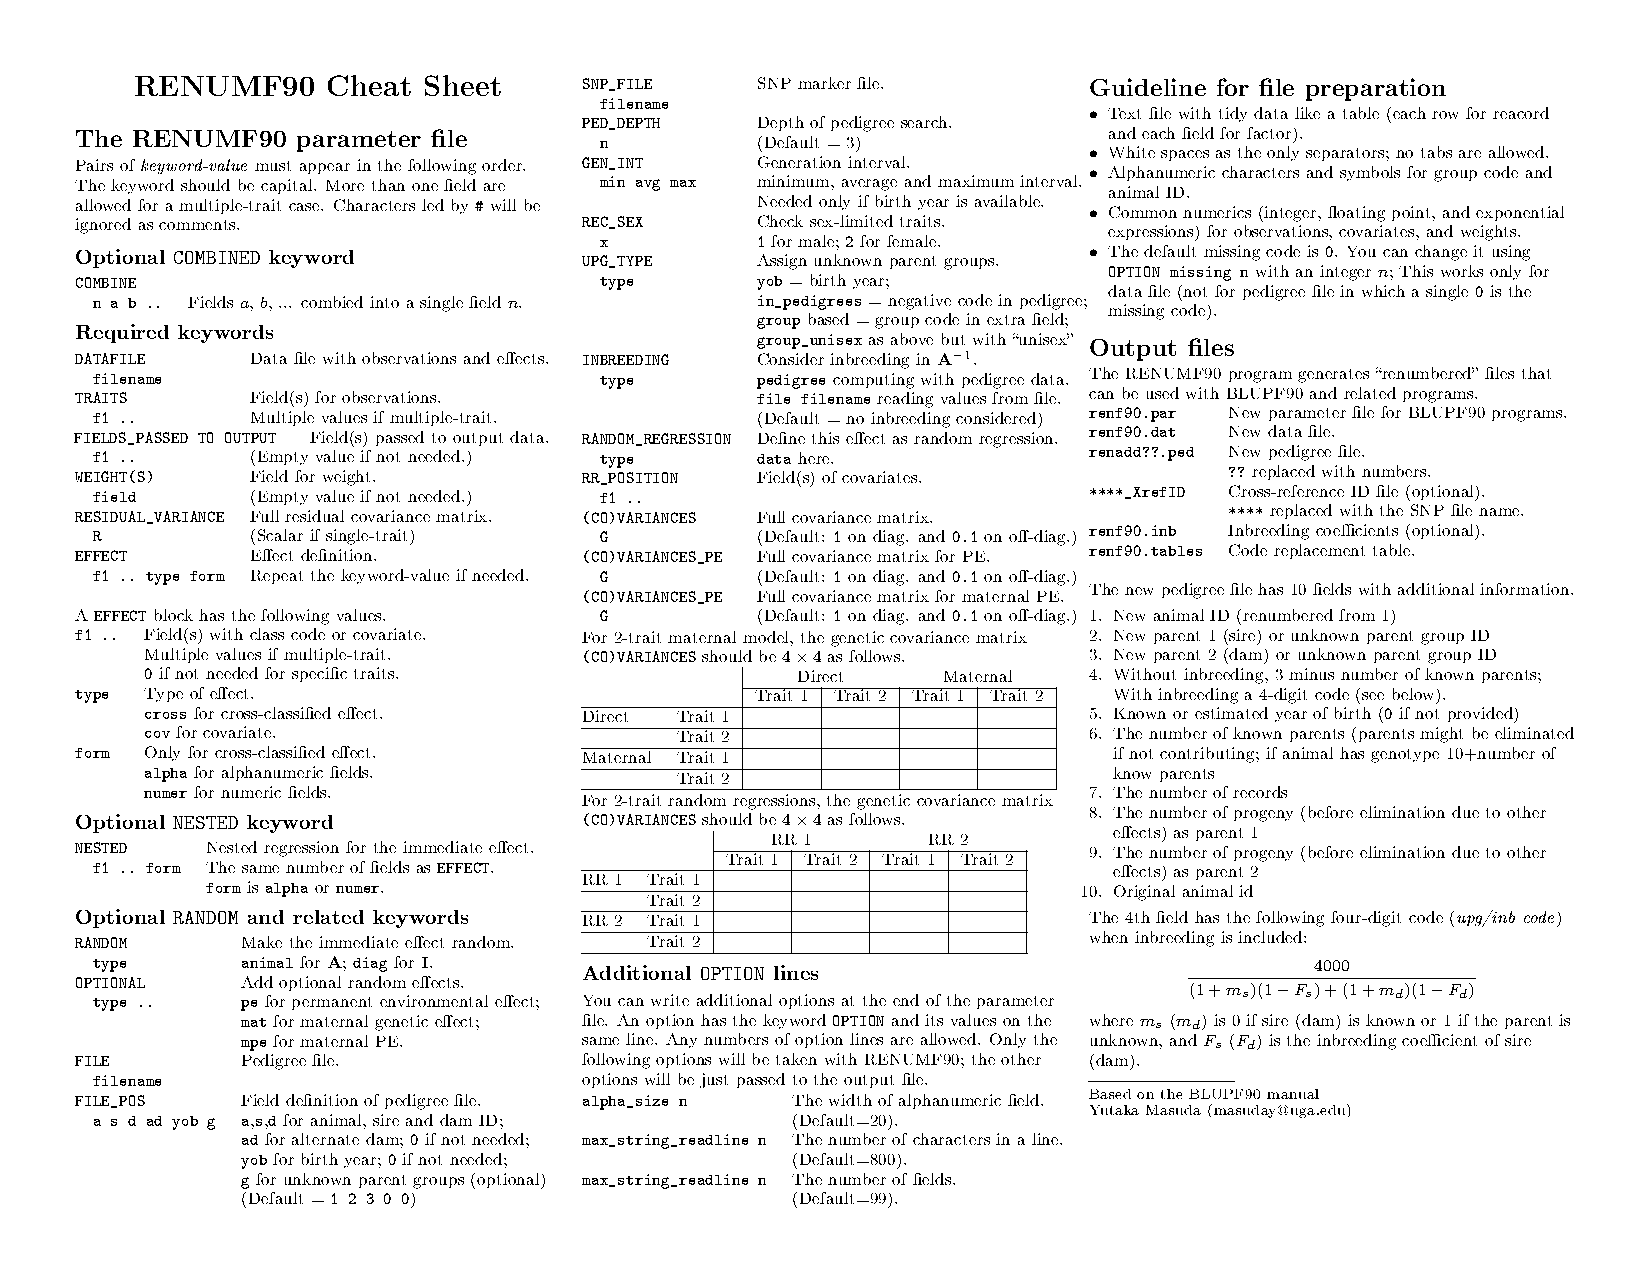
\includepdf[pages=-,angle=270]{blupsheet.pdf}

%\printindex

\end{document}
